\chapter{序列最小最优化算法(SMO)}

本节讨论支持向量机的实现问题,支持向量机的学习问题可以形式华为求解凸二次规划问题,这样的凸二次规划问题具有全局最优解。

\section{SMO算法}

SMO算法要解如下凸二次规划的对偶问题
\begin{eqnarray}
    & \min\limits_{\alpha} \ \ &\frac{1}{2}\sum\limits_{i=1}^{N}\sum\limits_{j=1}^{N}
    \alpha_i\alpha_jy_iy_j(x_i\cdot x_j)K(x_i,x_j)-\sum\limits_{i=1}^{N}\alpha_i\\
    & s.t. & \sum\limits_{i=1}^{N}\alpha_iy_i=0\\
    &      & 0\leqslant \alpha_i\leqslant C,\ \ i=1,2,\cdots,N
\end{eqnarray}

在这个问题中,变量是拉格朗日乘子,一个变量$\alpha_i$对应一个样本点$(x_i,y_i)$,变量的总数等于训练样本的容量$N$。

SMO算法是一种启发式算法,基本思路是:如果所有变量的解都满足次最优化问题的KKT条件,那么这个最优化问题的
解就得到了,因为KKT条件是该最优化问题的充分必要条件,否则,选择两个变量,固定其他变量,针对这两个变量构建一个二次规划
问题。这个二次规划问题关于这两个变量的解应该更接近原始二次规划问题的解。因为这会使得原始二次规范问题的目标函数值变小,
重要的是,这时子问题可以通过解析方法求解,这样就可以大大提高整个算法的计算速度。

子问题有两个变量,一个违反KKT条件最严重的那一个,另一个由约束条件自动确定。如此SMO算法将原问题不断分解为子问题并对子问题
求解,进而达到求解原问题的目的。

\section{两个变量的二次规划的求解方法}

不是一般性,假设选择的两个变量是$alpha_1$,$alpha_2$,其他变量$alpha_i(i=3,4,\cdots,N)$是固定的,于是SMO的最优化问题可以写成
\begin{eqnarray}
    & \min\limits_{\alpha_1,\alpha_2} & W(\alpha_1,\alpha_2)= \frac{1}{2}K_{11}\alpha^2_1+\frac{1}{2}K_{22}\alpha^2_2-\nonumber\\
    & & (\alpha_1+\alpha_2)+y_1\alpha_1\sum\limits_{i=3}^{N}y_i\alpha_i K_{i1}+y_2\alpha_2\sum\limits_{i=3}^{N}y_i\alpha_iK_{i2}\label{eq:7.101}\\
    & & s.t.\ \ \ \alpha_1y_1+\alpha_2y_2=-\sum\limits_{i=3}^{N}y_i\alpha_i=\varsigma\label{eq:7.102}\\
    & & 0\leqslant \alpha_i\leqslant C,\ \ i=1,2\label{eq:7.103}
\end{eqnarray}

其中$K_{ij}=K(x_i,x_j),i,j=1,2,\cdots,N$,$\varsigma$是常数,目标函数式(\ref{eq:7.101})中省略了不含$\alpha_1,\alpha_2$的常数项。

为了求解两个变量的二次规划问题,首先分析约束条件,然后在此约束条件下求极小。

由于只有两个变量$(\alpha_1,\alpha_2)$,约束可以用二维空间中的图形表示

\begin{figure}[H]
    \centering
    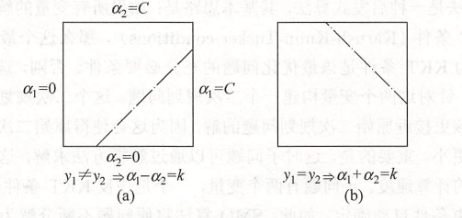
\includegraphics[scale=0.5]{figures/二变量优化问题.png}
    \caption{二变量优化问题}
    \label{二变量优化问题}
\end{figure}

不等式约束(\ref{eq:7.103})使得$(\alpha_1,\alpha_2)$在盒子$[0,C]\times [0,C]$内,等式约束(\ref{eq:7.103})使得
$(\alpha_1,\alpha_2)$在平行于盒子$[0,C]\times [0,C]$的对角线的直线上,因此要求的是目标函数在一条平行于对角线的线段上的最优值。
这使得两个变量的最优化问题称为实质上的单变量的最优化问题。不妨考虑为变量$\alpha_2$的最优化问题。

假设问题的初始可行解为$\alpha^{old}_1,\alpha^{old}_2$,最优解为$\alpha^{new}_1,\alpha^{new}_2$,并且假设在沿着约束方向
为经过剪辑时,$\alpha_2$的最优解为$\alpha^{new,unc}_2$。

由于$\alpha^{new}_2$需满足不等式约束(\ref{eq:7.103}),所以最优值$\alpha^{new}_2$的取值范围必须满足条件
\begin{equation}
    L\leqslant \alpha^{new}_2\leqslant H
\end{equation}

其中$L$和$H$是$\alpha^{new}_2$所在的对角线段的端点的界。如果$y_1\neq y_2$,则
\begin{equation}
    L=\max(0,\alpha^{old}_2-\alpha^{old}_1),\ \ H=\min(C,C+\alpha^{new}_2-\alpha^{new}_1)
\end{equation}

如果$y_1=y_2$,则
\begin{equation}
    L=\max(0,\alpha^{old}_2+\alpha^{old}_1-C),\ \ 
    H=\min(C,\alpha^{new}_2+\alpha^{new}_1)
\end{equation}

下面,首先沿着约束方向未经剪辑即为考虑不等式约束(\ref{eq:7.103})时,$\alpha_2$的最优解$\alpha^{new,unc}_2$;
然后再求剪辑后$\alpha_2$的解$\alpha^{new}_2$,我们用定律叙述这个结果,记
\begin{equation}
    g(x)=\sum\limits_{i=1}^{N}\alpha_iy_iK(x_i,x)+b
\end{equation}

令
\begin{equation}
    E_i=g(x_i)-y_i=(\sum\limits_{j=1}^{N}\alpha_jy_jK(x_j,x_i)+b)-y_i,\ \ i=1,2
\end{equation}

当$i=1,2$时,$E_i$为函数$g(x)$对输入$x_i$的预测值与真实输出$y_i$之差。

\subsection*{定理}
\begin{theorem}
    最优化问题(\ref{eq:7.101})$\sim$(\ref{eq:7.103})沿着约束方向未经剪辑时的解时
    \begin{equation}
       \alpha^{new,unc}_2=\alpha^{old}_2+\frac{y_2(E_2-E_1)}{\eta}
    \end{equation}

    其中,

    \begin{equation}
        \eta=K_{11}+K_{22}-2K_{12}=\Vert \phi(x_1)-\phi(x_2)\Vert^2
    \end{equation}

    $\phi(x)$是输入空间到特征空间的映射。

    经过剪辑后$\alpha_2$的解是
    \begin{equation}
        \alpha^{new}_2=
        \begin{cases}
            &H, \ \ \ \ \ \ \ \ \ \alpha^{new,unc}_2>H\\
            &\alpha^{new,unc}_2,\ \ \ \  L\leqslant \alpha^{new,unc}_2\leqslant \alpha^{new,unc}_2\\
            & L,\ \ \ \ \ \ \ \ \ \alpha^{new,unc}_2\leqslant L
        \end{cases}
    \end{equation}

    由$\alpha^{new}_2$求得$\alpha^{new}_1$是
    \begin{equation}
        \alpha^{new}_1=\alpha^{old}_1+y_1y_2(\alpha^{old}_2-\alpha^{new}_2)
    \end{equation}
\end{theorem}

\section{变量的选择方法}

SMO算法在每个子问题中选择两个变量优化,其中至少一个变量是违反KKT条件的。

\subsection*{第一个变量的选择}

SMO选择第1个变量的过程称为\textsl{外层循环}。外层循环在训练样本中违反KKT条件最严重的样本点。并将其对应的变量
作为第1个变量。具体地,检验训练样本点是否满足KKT条件,即
\begin{equation}
    \alpha_i=0\Leftrightarrow y_ig(x_i)\geqslant 1
\end{equation}
\begin{equation}
    0<\alpha_1<C\Leftrightarrow y_ig(x_i)=1
\end{equation}
\begin{equation}
    \alpha_i=C\Leftrightarrow y_ig(x_i)\leqslant 1
\end{equation}

其中,$g(x_i)=\sum\limits_{j=1}^{N}\alpha_jy_jK(x_i,x_j)+b$。

该检验是在$\epsilon$范围内进行的。在检验过程中,外层循环首先遍历所有条件$0\leqslant \alpha_i<C$的样本点
,即间隔边界上的支持向量点,检验它们是否满足KKT条件。如果这些样本点都满足KKT条件,那么遍历整个训练集,检验它们是否满足KKT条件。

\subsection*{第二个变量的选择}

SMO选择第2个变量的过程称为\textsl{内层循环}。假设外层循环中已经找到了第1个变量$\alpha_1$,现在要在内层循环中
要找到第2个变量$\alpha_2$,第2个变量选择的标准死后希望能使得$\alpha_2$有足够大的变化。

\subsection*{计算阈值$b$和差值$E_i$}

\section{SMO算法}

输入:训练数据集$T=\{(x_1,y_1),(x_2,y_2),\cdots,(x_1N,y_N)\}$;

输出:近似解$\hat{\alpha}$;

\begin{enumerate}[itemindent=2em]
    \item[(1)] 取初值$\alpha^{(0)}=0$,令$k=0$;
    \item[(2)] 选取优化变量$\alpha^{(k)}_1$,$\alpha^{(k)}_2$,解析求解两个变量的最优化问题(\ref{eq:7.101})$\sim$(\ref{eq:7.103})。
    求得最优解$\alpha^{k+1}_1$,$\alpha^{k+1}_2$,更新$\alpha$为$\alpha^{(k+1)}$。
    \item[(3)] 若在精度$\epsilon$范围内满足停机条件
    \begin{equation}
        \sum\limits_{i=1}^{N}\alpha_iy_i=0,\ \ 0\leqslant \alpha_i\leqslant C,\ \ i=1,2,\cdots,N\\
    \end{equation}

    \begin{equation}
        y_i\cdot g(x_i)=
        \begin{cases}
            & \geqslant 1, \ \ \ \{x_i|\alpha_i=0\}\\
            & = 1, \ \ \ \{x_i|0<\alpha_i<C\}\\
            & \leqslant 1, \ \ \ \{x_i|\alpha_i=C\}\\
        \end{cases}
    \end{equation}

    (其中$ g(x_i)=\sum\limits_{j=1}^{N}\alpha_jy_jK(x_j,x_i)$)

    则转(4),否则令$k=k+1$,转(2)。

    \item[(4)] 取$\hat{\alpha}=\alpha^{k+1}$
\end{enumerate}